\documentclass{standalone}
\usepackage{tikz,pgfplots,calc}
\usetikzlibrary{positioning,calc}
\usetikzlibrary{arrows}
\usepackage{tkz-euclide}
\usepackage{amsmath}
\usetkzobj{all}

\tikzset{
  mynode/.style = {draw, minimum width = .4cm, minimum height = 2cm}}

\begin{document}
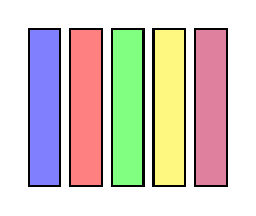
\begin{tikzpicture}[>=stealth', thick]


% \node [lable=below:a, drw] at (10, 10);
\node[mynode, fill = blue!50] (n1) {};
\node[mynode, fill = red!50, anchor = west, right=.1cm of n1.east] (n2) {};
\node[mynode, fill = green!50, anchor = west, right=.1cm of n2.east] (n3) {};
\node[mynode, fill = yellow!50, anchor = west, right=.1cm of n3.east] (n4) {};
\node[mynode, fill = purple!50, anchor = west, right=.1cm of n4.east] (n5) {};

% \node [scale = .9, anchor = center] at (1.1, -1.3) {$\mathbf{X}_{\text{train}} = [\mathbf{x}_1, \mathbf{x}_2, \dots]$};
\end{tikzpicture}
\end{document}